\chapter{Estimating the beamline}
\textit{Definition of luminous region, its importance in Alignment and Calibration, luminosity and other stuff}
The beamline is defined as the region where the two beams of particles collide, as depicted in Figure \ref{fig:luminous-region}. The position of the beamline corresponds to the area where the primary vertices of these collisions are formed, hence beamline and luminous region are treated as synonyms.



\begin{figure}
    \centering
    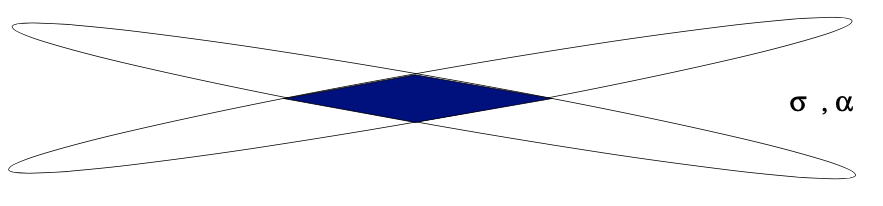
\includegraphics[width=\textwidth]{figures/luminous_region.png}
    \caption{Luminous regions (blue), given the overlap of two bunches}
    \label{fig:luminous-region}
\end{figure}

%\begin{figure}
%    \centering
%    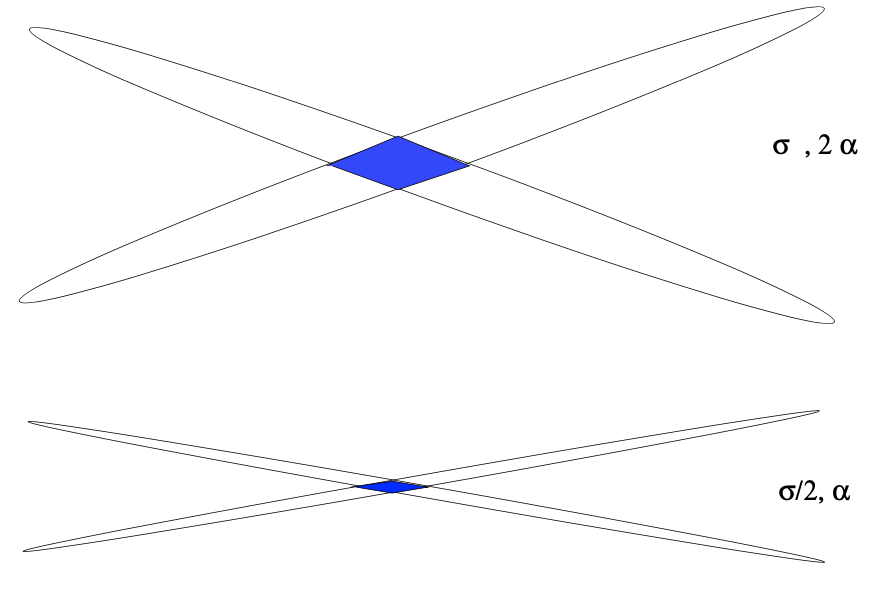
\includegraphics[width=\textwidth]{figures/luminous_region_var.png}
%    \caption{Luminous regions (blue), given the overlap of two bunches with different parameters (width \sigma and crossing angle \alpha) with respect to Figure \ref{fig:luminous-region}}
%    \label{fig:luminous-region-var}
%\end{figure}


Understanding the position of the beamline is critical for two main reasons:
\begin{itemize}
\item Luminosity Estimation Correction: The luminosity of an experiment is closely tied to the position of the beamline. If the luminosity estimate is based on an incorrect beamline position, the resulting measurements will be skewed. To provide accurate online luminosity estimates, a method is needed to correct for errors in the beamline position. This involves implementing a data point that continuously monitors the real-time beamline position to adjust the luminosity calculation accordingly.
\item Track Reconstruction Algorithms: The current algorithms for track reconstruction has relied until 2024 on a predefined, "hardcoded" position of the beamline. If this position is not updated accurately, the precision of the track reconstruction can be compromised. A real-time estimation of the beamline position can enhance the efficiency of track reconstruction.
\end{itemize}

As already stated various times, both HLT$1$ and HLT$2$ PVs reconstruction algorithms use the beamline position as an input. Until 2023, the collobartion relied for this information on a configuration file named ``InteractionRegion", which was manually updated when necessary. In February 2024, the LHCb developed ``BeamSpot Monitor", a tool used for the automatically update of the ``InteractionRegion" configuration file.  This tool operates in the Alignment \& Calibration phase of the online trigger, accumulating statistics and booking histograms of the reconstructed PVs. Once the histograms are available, the mean and covariance are calculated, providing an estimation of the beamline position to both HLT$1$ and HLT$2$. This iterative procedure is computationally expensive and relies on the PVs reconstructed during HLT$1$.

In this chapter, we explore an innovative approach to determining the beamline position in real-time without relying on traditional track reconstruction algorithms. This method provides accurate information on the beamline position, facilitating timely corrections for both luminosity estimation and track reconstruction. Through this approach, we aim to improve the overall accuracy and efficiency of the experiment's data analysis processes.

It was already shown in an earlier work\cite{dan}, that the counters implemented for the luminosity are sensible to beamline displacement. An example of this sensibility is depicted in Figure \ref{fig:z_lumi_dependency}, where one can clearly see how the mean of the outer counters per event is slightly different depending on the luminus region position. 

\begin{figure}
    \centering
    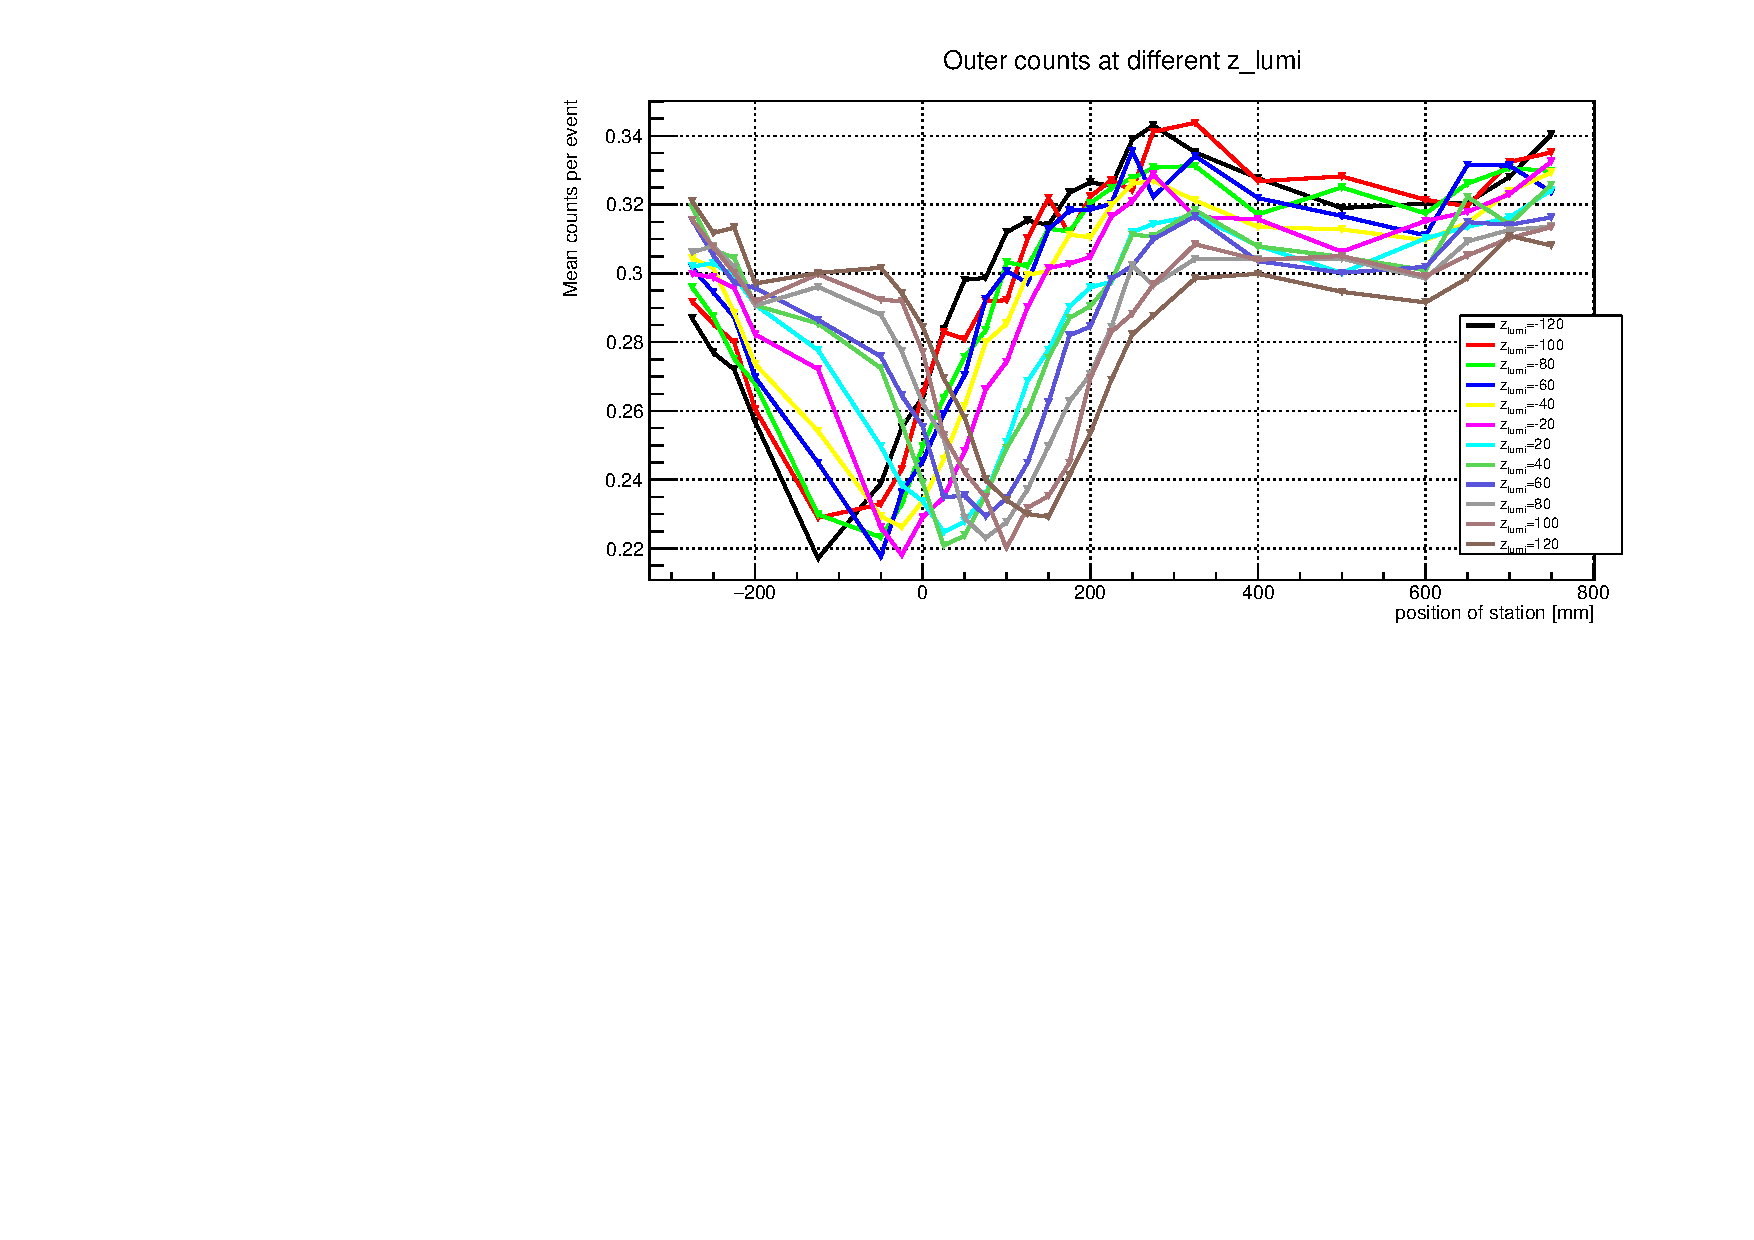
\includegraphics[width=\textwidth]{figures/z_lumi_dependency.pdf}
    \caption{Mean cluster counts per event of the outer counters as a function of the z position of the VELO station on which the counter is implemented. Each different line represents a different simulation on which the beamline position is displaced as indicated in the legend of the Figure.}
    \label{fig:z_lumi_dependency}
\end{figure}

In this chapter, I study a way to combine the 208 implemented counters to give an estimation of the beamline position in each component x, y, and z. A possibility relies on leveraging the capabilities of a dimensionality reduction technique called Principal Component Analysis, which allows to transform the data in the 208-dimensional space to a space of fewer dimensions. The hope is that the parameters of the beamline will be depenent from some of the features extracted with this method. In the next sections I will present the technique, the Monte Carlo simulations used to study the estimators and some tests on real collision data.

%The Principal Component Analysis is not the only possibility 


\section[The Principal Component Analysis]{The Principal Component Analysis $\bigl($PCA$\bigr)$}

The Principal Component Analysis (PCA) is a widely used statistical technique for dimensionality reduction, feature extraction, and data compression. It involves transforming a dataset into a new coordinate system with a linear orthogonal transformation designed to maximize the variance along the first principal component (the first coordinate of the transformed system), with the subsequent components containing successively decreasing variance.
An intuition and visualizationof this transformation is given in Figure \ref{fig:pca}.

\begin{figure}
    \centering
    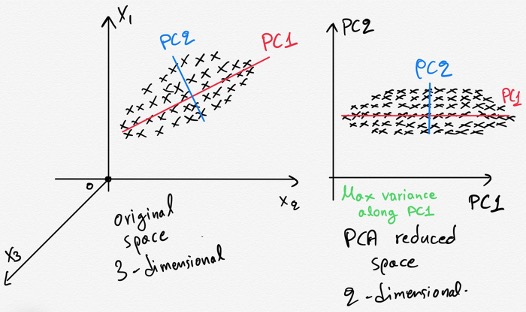
\includegraphics[width=0.8\textwidth]{figures/pca.jpg}
    \caption{Schematic understanding of the Principal Component Analysis: suppose to have a 3 dimensional dataset (right). We can transform this space in a 2 dimensional one, with a new basis of two variables given by the two first Principal Components (PC1 and PC2), ordered by the variance captured by the projection of the data on that component.}
    \label{fig:pca}
\end{figure}


Let $\mathbf{X}$ be a data matrix with column-wise zero empirical mean (the sample mean of each column has been shifted to zero), where $n$ are the number of samples and $p$ the number of features. PCA identifies $l$ principal components (where $l \leq p$) that capture the most variance in the data.

Mathematically, PCA transforms the data by finding a set of size $l$ of $p$-dimensional vectors of weights, or coefficients, $\mathbf{w}_{(k)} = (w_1, \ldots, w_p)_{(k)}$, that map each row vector $\mathbf{x}_{(i)}$ of $\mathbf{X}$ to a new vector of ordered principal component scores $\mathbf{t}_{i} = (t_1, \ldots, t_l)_{(i)}$, defined as:

\begin{equation}
{t_{k}}_{(i)} = \mathbf{x}_{(i)} \cdot \mathbf{w}_{(k)} \quad \text{for} \quad i = 1, \ldots, n \quad k = 1, \ldots, l
\end{equation}

The goal is to maximise the variance along each principal component PC, with each coefficient vector \(\mathbf{w}\) constrained to be a unit vector. Typically, \(l\) is selected to be less than \(p\) to reduce dimensionality.


The first PC $t_{1}$ maximises the variance of the dataset, thus the weight vector \(\mathbf{w}_{(1)}\) must satisfy the following condition:

\begin{equation}
\mathbf{w}_{(1)} = \arg \max_{\|\mathbf{w}\| = 1} \left\{ \sum_{i=1}^{n} \left( \mathbf{x}_{(i)} \cdot \mathbf{w} \right)^2 \right\}.\label{argmax}
\end{equation}

Let's break it down to the single pieces: 
\begin{itemize}
    \item $\mathbf{x}_{(i)} \cdot \mathbf{w}$ represents the projection of a data entry on a direction in the feature space (208-dimensional) described by a vector $ \mathbf{w}$;
    \item $ \sum_{i=1}^{n} \left( \mathbf{x}_{(i)} \cdot \mathbf{w} \right)^2$ is the variance of the projection of the whole dataset on the direction described by the vector $ \mathbf{w}$;
    \item $\|\mathbf{w}\| = 1$ ensures that $\mathbf{w}$ is properly normalised as a unit vector;
    \item the $\arg \max$ operation finds the vector $\mathbf{w}$, such that the projection of the dataset on this vector has the greatest variance, with respect to all the other projections.
\end{itemize}

The condition \ref{argmax} can be rewritten in matrix form as:

\begin{equation}
\mathbf{w}_{(1)} = \arg \max_{\|\mathbf{w}\| = 1} \left\{ \|\mathbf{Xw}\|^2 \right\} = \arg \max_{\|\mathbf{w}\| = 1} \left\{ \mathbf{w}^{\mathsf{T}} \mathbf{X}^{\mathsf{T}} \mathbf{Xw} \right\}.
\end{equation}

Incorporating the normalisation in the analytical form, we get a more straightforward expression:

\begin{equation}
\mathbf{w}_{(1)} = \arg \max \left\{ \frac{\mathbf{w}^{\mathsf{T}} \mathbf{X}^{\mathsf{T}} \mathbf{Xw}}{\mathbf{w}^{\mathsf{T}} \mathbf{w}} \right\}.\label{first_weight}
\end{equation}

The quantity to maximise is recognised as a Rayleigh quotient\cite{horn13}. A positive semidefinite matrix such as $\mathbf{X}^{\mathsf{T}} \mathbf{X}$ has the maximum possible Rayleigh quotient value as its largest eigenvalue, which occurs when $\mathbf{w}$ is the corresponding eigenvector\cite{parlett1998symmetric}.


With $\mathbf{w}_{(1)}$ found, the first PC score of a data vector $\mathbf{x}_{(i)}$ can be calculated as:

\begin{equation}
t_{1(i)} = \mathbf{x}_{(i)} \cdot \mathbf{w}_{(1)}.\label{first_score}
\end{equation}

In order to find subsequent components, the contribution given by $\mathbf{t}_{(1)}$ must be subtracted from the original dataset. This procedure ensures that the subsequent PC focuses on the variance that remains in the data. Iterating the reasoning, the $k$-th PC is found by subtracting the contributions given by the first $k-1$ components. We can hence define a residual matrix $\mathbf{\hat{X}}_{k}$

\begin{equation}
\mathbf{\hat{X}}_{k} = \mathbf{X} - \sum_{s=1}^{k-1} \mathbf{X} \mathbf{w}_{(s)} \mathbf{w}_{(s)}^{\mathsf{T}},\label{dim_red_tran}
\end{equation}
that represents the projection of the data on a subspace orthogonal to the first $k-1$ components.

Creating this matrix, the problem reduces to the case just discussed, with the solution for $\mathbf{w}_{(k)}$ being the eigenvector with the highest corresponding eigenvector of the space $\mathbf{\hat{X}}_{k}^\mathsf{T}\mathbf{\hat{X}}_{k}$. But this eigenvector of the residual space $\mathbf{\hat{X}}_{k}$ is the $k$-th  eigenvector of the $\mathbf{X}^{\mathsf{T}} \mathbf{X}$ space since eigenvectors corresponding to distinct eigenvalues are always orthogonal to one another, as stated by the spectral theorem.

This allows us to generalise \eqref{first_score} to a general $k$-th PC score:
\begin{equation}
t_{k(i)} = \mathbf{x}_{(i)} \cdot \mathbf{w}_{(k)}.\label{score}
\end{equation}


%\mathbf{w}_{(k)} = \operatorname{arg\,max}_{\|\mathbf{w}\| = 1} \left\{\|\mathbf{\hat{X}}_{k} \mathbf{w}\|^{2}\right\} = \operatorname{arg\,max} \left\{ \frac{\mathbf{w}^{\mathsf{T}} \mathbf{\hat{X}}_{k}^{\mathsf{T}} \mathbf{\hat{X}}_{k} \mathbf{w}}{\mathbf{w}^{\mathsf{T}} \mathbf{w}} \right\}.


%The optimal value for the Rayleigh quotient is given by the maximum eigenvalue of the positive semidefinite matrix $\mathbf{X}^{\mathsf{T}} \mathbf{X}$, with the corresponding eigenvector providing the weight vector $\mathbf{w}_{(k)}$. This leads to a recursive procedure, where each subsequent principal component derives from a modified dataset.



Hence, the weights $\mathbf{w}_{(k)}$ of the PCA are found by diagonalizing the sample covariance matrix $\mathbf{S}$ of the data $\mathbf{X}$, being this defined as:

\begin{equation}
\mathbf{S} =  \frac{1}{n-1} \mathbf{X}^{\mathsf{T}} \mathbf{X} -  \mathbf{\mu_X}^{\mathsf{T}}\mathbf{\mu_X}= \frac{1}{n-1} \mathbf{X}^{\mathsf{T}} \mathbf{X},
%\operatorname {K} _{X_{i}X_{j}}=\operatorname {cov} [X_{i},X_{j}]=\operatorname {E} [(X_{i}-\operatorname {E} [X_{i}])(X_{j}-\operatorname {E} [X_{j}])]
\end{equation}
since $\mathbf{X}$ has column-wise zero empirical mean $\mathbf{\mu_X}=\vec{0}$. 
In order to find the right order of the PCs, the eigenvectors of $\mathbf{S}$ are then ordered by the magnitude of their eigenvalues, with the largest eigenvalue corresponding to the direction with the most variance in the data (first PC). The (normalized) eigenvalues represent the amount of variance explained by each PC.


\begin{algorithm}
\caption{Principal Component Analysis (PCA)}
\begin{algorithmic}[1]
    \STATE \textbf{Input:} Dataset \(\mathbf{X}\), with \(n\) samples and \(p\) features, and the desired number of principal components \(l\).

    \STATE \textbf{Step 1:} Compute the covariance matrix \(\mathbf{S}\) of the dataset:
    \begin{equation*}
    \mathbf{S} = \frac{1}{n - 1} \mathbf{X}^{\mathsf{T}} \mathbf{X}.
    \end{equation*}

    \STATE \textbf{Step 2:} Calculate the eigenvectors \(\mathbf{w}_{(k)}\) and eigenvalues \(\lambda_k\) of the covariance matrix \(\mathbf{S}\).

    \STATE \textbf{Step 3:} Sort the eigenvectors \(\mathbf{w}_{(k)}\) by their corresponding eigenvalues in descending order.

    \STATE \textbf{Step 4:} Calculate the first \(l\) principal components for each sample \(\mathbf{x}_{(i)}\):
    \begin{equation*}
    {t_{k}}_{(i)} = \mathbf{x}_{(i)} \cdot \mathbf{w}_{(k)} \quad \text{for} \quad i = 1, \ldots, n \quad k = 1, \ldots, l.
    \end{equation*}
    
    \STATE \textbf{Output:} The principal component scores \(\mathbf{t}\), and the principal component vectors \(\mathbf{w}\).
\end{algorithmic}
\end{algorithm}


The complete principal component decomposition of the data matrix $\mathbf{X}$ can be given in matrix form by:

\begin{equation}
\mathbf{T} = \mathbf{X} \mathbf{W},
\end{equation}

where $\mathbf{W}$ is a $p \times p$ matrix containing the eigenvectors of $\mathbf{S}$.



\section{The Monte Carlo simulations}
To assess the relationship between measured rates on both luminosity and beamline position, I perform feasibility studies using official LHCb simulations. These simulations allow us to evaluate how variations in luminosity and beamline parameters impact the detector's response.

The LHCb simulation workflow encompasses multiple software applications, each responsible for a specific task. The generation of primary particles from proton-proton collisions is handled by the \textsc{Pythia} package \cite{Sj_strand_2006}, a versatile event generator. Particle decays are simulated through the \textsc{EvtGen} framework \cite{Lange:2001uf}, while the propagation of particles through the detector is modelled with the \textsc{Geant4} toolkit \cite{Agostinelli:2002hh}, which includes a detailed geometric description of all detector components.

All these tasks are managed by the \textsc{Gauss} application \cite{Miglioranzi:1322402}, which integrates the different simulation stages. \textsc{Gauss} also manages various luminosity-related parameters such as pile-up, luminous region position (in \(x, y,\) and \(z\)), its width, beam crossing angle, and beamline inclination.

The sub-detectors' responses to simulated particles are generated by the \textsc{Boole} application, which handles signal digitisation in the same format as the actual experiment's data acquisition system. After digitisation, the simulated data follow the same processing path as real data, passing through the same trigger, reconstruction, and analysis software. The trigger application, known as \textsc{Moore}, includes algorithms for both high-level triggers. 

To investigate the impact of the VELO cluster counters on the beamline and luminosity estimations, a software version of the firmware for the luminosity counters was implemented in the \textsc{Moore} framework. This modification allows for the emulation of the hardware's functionality, enabling studies of how changes in beamline parameters affect the counters' readings.

Multiple simulation scenarios were conducted to examine the effects of different settings for instantaneous luminosity and beamline parameters. All simulations are based on Minimum Bias events, representing generic pp inelastic collisions. They use the LHCb Upgrade I detector simulation with a center-of-mass energy of $\sqrt{s} = \SI{13.6}{\tera\eV}$ and a bunch spacing of \SI{25}{\nano\second}. Unless specified otherwise, each simulation analyzed $10^5$ events. The simulations covered various configurations:

\begin{enumerate}

    \item[(i)] A scan of the luminous region's mean $z$-position from \SI{-120}{\milli\meter} to \SI{120}{\milli\meter} at $\Delta z=\SI{20}{\milli\meter}$ steps relative to the LHCb reference frame, with $\nu = 7.6$, $x = \SI{0}{\milli\meter}$, and $y = \SI{0}{\milli\meter}$, in MagDown configuration. A file for each nominal position is produced.

    \item[(ii)] A scan of the luminous region's mean $y$-position from \SI{-1.5}{\milli\meter} to \SI{1.5}{\milli\meter} at $\Delta y =\SI{0.5}{\milli\meter}$ steps relative to the LHCb reference frame, with $\nu = 7.6$, $x = \SI{0}{\milli\meter}$, and $z = \SI{0}{\milli\meter}$, in MagDown configuration. A file for each nominal position is produced.

     \item[(iii)] A scan of the luminous region's mean $x$-position from \SI{-1.5}{\milli\meter} to \SI{1.5}{\milli\meter} at $\Delta x =\SI{0.5}{\milli\meter}$ steps relative to the LHCb reference frame, with $\nu = 7.6$, $y = \SI{0}{\milli\meter}$, and $z = \SI{0}{\milli\meter}$, in MagDown configuration. A file for each nominal position is produced.

     \item[(iv)] A scan of event pile-up \(\nu\) from $3.8$ to $35.8$, corresponding to an instantaneous luminosity range of \SI{1e33}{\per\centi\meter\squared\per\second} to \SI{9.4e33}{\per\centi\meter\squared\per\second}. The mean position of the interaction region was set to $(0.0, 0.0, 0.0)$ mm. Simulations were conducted with both MagDown and MagUp magnet configurations. A file for each nominal position is produced.

\end{enumerate}


The beamline position is defined as the distribution of the PVs, hence the value reported on the bullet list above indicate the average position of the PVs. The luminous region is spread for about \SI{30}{\milli\meter} in the $z$ component, while it has a width of \SI{15}{\micro\meter} in both the $x$ and $y$ directions.  

These simulations are used for various purposes. 
\begin{itemize}
\item The simulations in (i), (ii), (iii) are used to construct datasets on which the PCA is performed. As explained in the previous section, the PCA furnish a new set of coordinates such that the first coordinate describes the direction of maximal variance of the dataset. If we can construct a dataset in which the only varying component is the beamline position along one direction and execute the PCA on that dataset, some of the first PCs should be quantities depending on the beamline position. This procedure is explained in detail in the next section.
\item The simulations in (iv) are used to check for the dependency of the beamline estimators to the luminosity. If the luminosity is linear in the counter as explained in Chapter \ref{chap:luminosity}, it follows straightforwardly that the luminosity will also bias the beamline estimation linearly. This MC simulations are used to check this behaviour.
\end{itemize}

From each one of the simulation files in (i), (ii), (iii) we produce a tuple containing 212 features:
\begin{itemize}
    \item The event number: it is the index of the tuple indicating the label of the event. It is an integer running from $0$ to $10^5$.
    \item $x$-position [mm]: the $x$ position of the beamline reconstructed as the mean of PVs. It is a float number that can assume 7 possible values: $-1.5$, $-1.0$, $-0.5$, $0.0$, $0.5$, $1.0$, $1.5$
    \item $y$-position [mm]: the $y$ position of the beamline reconstructed as the mean of PVs. It is a float number that can assume 7 possible values: $-1.5$, $-1.0$, $-0.5$, $0.0$, $0.5$, $1.0$, $1.5$
    \item $z$-position [mm]: the $z$ position of the beamline reconstructed as the mean of PVs. It is a float number that can assume 13 possible values: \\
    $-120.0$, $-100.0$, $-80.$, $-60.0$, $-40.0$, $-20.0$, $0.0$, $20.0$, $40.0$, $60.0$, $80.0$, $100.0$, $120.0$
    \item the 208 counters: the remaining 208 features indicate the number of clusters counted by each specific counter in that event. It is an integer number that can assume any positive value.
\end{itemize}

Subsequently, we append together the tuples files created from (i), (ii) and (iii), in order to obtain three different files, one relative to each position $x$, $y$ or $z$. We end up with three tuples: the ones for $x$ and $y$ contain 600 thousand events, while the one for $z$ contain 1.2 million events. 

In order to create the datasets used to estimate the Principal Components we have to perform one further step.
The quantities read in the firmware are the rates of clusters, hence we need to create a dataset in which the feature of the 208 counters are not the counts of clusters, but rather the mean number of clusters per event. This can be done mediating over $N$ entries of the dataset. The choice of this integration constant is no matter to take lightly. The counters are read in firmware once every $3$ seconds, meaning that at a crossing rate of \SI{40}{\mega\hertz} they integrate 120 million events. Unfortunately, we do not have such high statistics in the Monte Carlo, meaning that this integration constant needs to be set lower. It was decided to have 5 points per position in each dataset, meaning that the integration constant is set to $10^5/5=20\times10^3$. Therefore, we create the final tuples on which we perform the PCA by integrating chunks of $20000$ events at the same nominal position. By doing so, we create a dataset for each position containing 30 entries for $x$ and $y$ and 60 entries for $z$. A schematic of this last procedure is depicted in Figure \ref{fig:tabular_dataset}. 

\begin{figure}
    \centering
    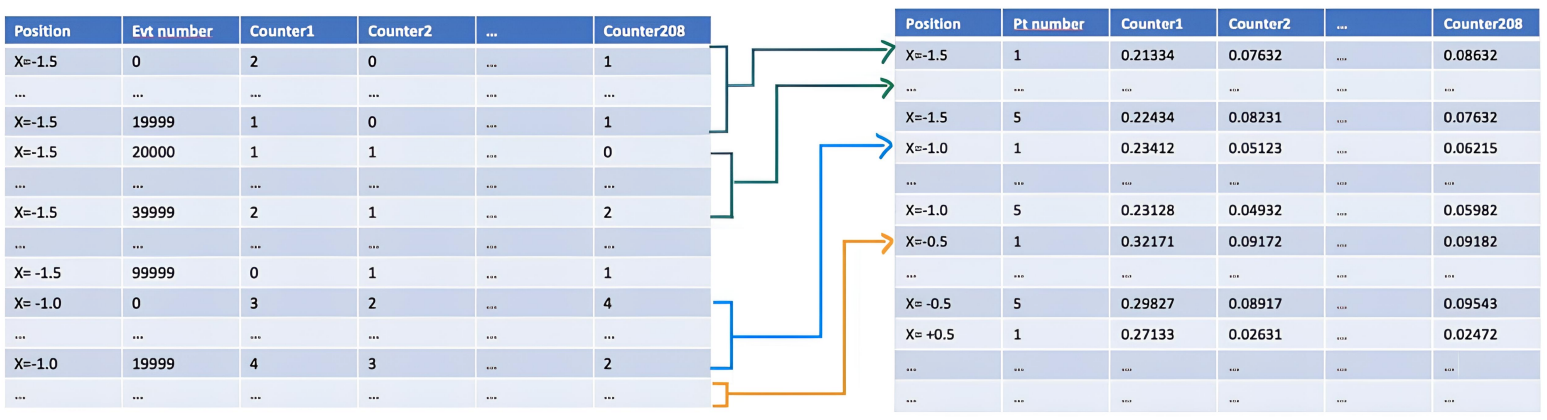
\includegraphics[width=\textwidth]{figures/tabular_dataset.png}
    \caption{Scheme of the last step in the creation of the tabular dataset used for estimating the PCA. An example regarding the x dataset is depicted. In the table on the left the dataset containing the raw events obtained from the simulation files are depicted. Notice that we have 100 thousand points for each nominal position and that the variables Counter1, Counter2, etc. indicate an integer, i.e. the number of clusters counted in that specific event. The tabular dataset on the right is obtained by integrating chunks of 20 thousand events at the same nominal position. Notice that in the dataset on the right we have 5 points per position, and that the features indicating the counters are float values that indicate the \textit{rate} of the counters, i.e. the mean number of clusters per event.}
    \label{fig:tabular_dataset}
\end{figure}

The very last step of this dataset creation procedure involves splitting each dataset in two, in order to create the final datasets: 
\begin{itemize}
    \item the train dataset: in the training dataset only the first 2 points per position are kept. We end up with a dataset containing 12 entries for $x$ and $y$, and $24$ entries for $z$. This dataset is used to estimate the weights $\mathbf{w}_{(k)}$ as described in the previous section.
    \item the test dataset: in the test dataset the last 3 points per position are stored. These points are used to estimate the scores $\mathbf{t}_{(i)}$ and asses their relationship with the beamline position. By fitting this yet-to-discover relationship we can also calculate the residuals in order to estimate the resolution of the estimators.
\end{itemize}


\section{Creating the estimators on MC}

We want to construct three different quantities $\hat{x}$, $\hat{y}$, $\hat{z}$ to estimate the beamline position components using $l$ scores $t_k$ derived with the PCA algorithm.
\begin{align}
    \hat{x} &= \hat{x}(t^x_1, \dots, t^x_l)_{(k)} \\
    \hat{y} &= \hat{y}(t^y_1, \dots, t^y_l)_{(k)} \\
    \hat{z} &= \hat{z}(t^z_1, \dots, t^z_l)_{(k)} 
\end{align} 

Each one of the scores $t_k$ is described by \eqref{score}, hence we need to properly define $\mathbf{x}_{(i)}$ and $\mathbf{w_{(k)}}$. The $\mathbf{x}_{(i)}$ vector is a p-dimenisonal vector containing the mean counts per events on each one of the p implemented counters. The  $\mathbf{w_{(k)}}$ is the vector of weights for calculating the $k$-th component with the PCA algorithm and we will use the MC to estimate them. 
As anticipated, we need to construct a dataset on which the only varying component is the beamline position along one of the direction. This can be done using the simulations (i), (ii), (iii) described in the previous section. 


Let $\mathbf{c}=(c_1, \dots, c_p)$ be the counts registered by each counter $k$ with $k$ iterating from $1$ to $p=208$. Let $\mathbf{\mu}=(\mu_1, \dots, \mu_p)$ be the mean counts per event associated to each counter $k$ and $\mathbf{\Sigma}$ the $p\times p$ covariance matrix describing the correlation between the counters. Since it is a counting experiment, the assumption is that the variable $\mathbf{c}$ follows a multivariate Poisson distribution described by the parameters $\mathbf{\mu}$ and $\mathbf{\Sigma}$. We introduce the parameter $\mathbf{x}=(x,y,z)$ representing the beamline position as a further parameter of the distribution. 
%and we porform a change of variable from the raw counts $\mathbf{c}$ to the mean counts per event $\mathbf{m}$.
In the central limit theorem (CLT), this distribution can be approximated with a multivariate gaussian of the form 
\begin{equation}
    P(\mathbf{c} ; \mathbf{\mu},\mathbf{\Sigma} |\mathbf{x}) = \frac{\exp \bigl(-\frac{1}{2}(\mathbf{c}-\mathbf{\mu})^{\mathsf{T}}\mathbf{\Sigma}^{-1}(\mathbf{c}-\mathbf{\mu})\bigr)}{\sqrt{(2\pi)^p\det\mathbf{\Sigma}}}
\end{equation} 


The counters position on each station of the VELO furnish a base for a conceptual 208-dimensional vector space. Each one of these counter is a feature $p$. 


\begin{figure}
    \centering
    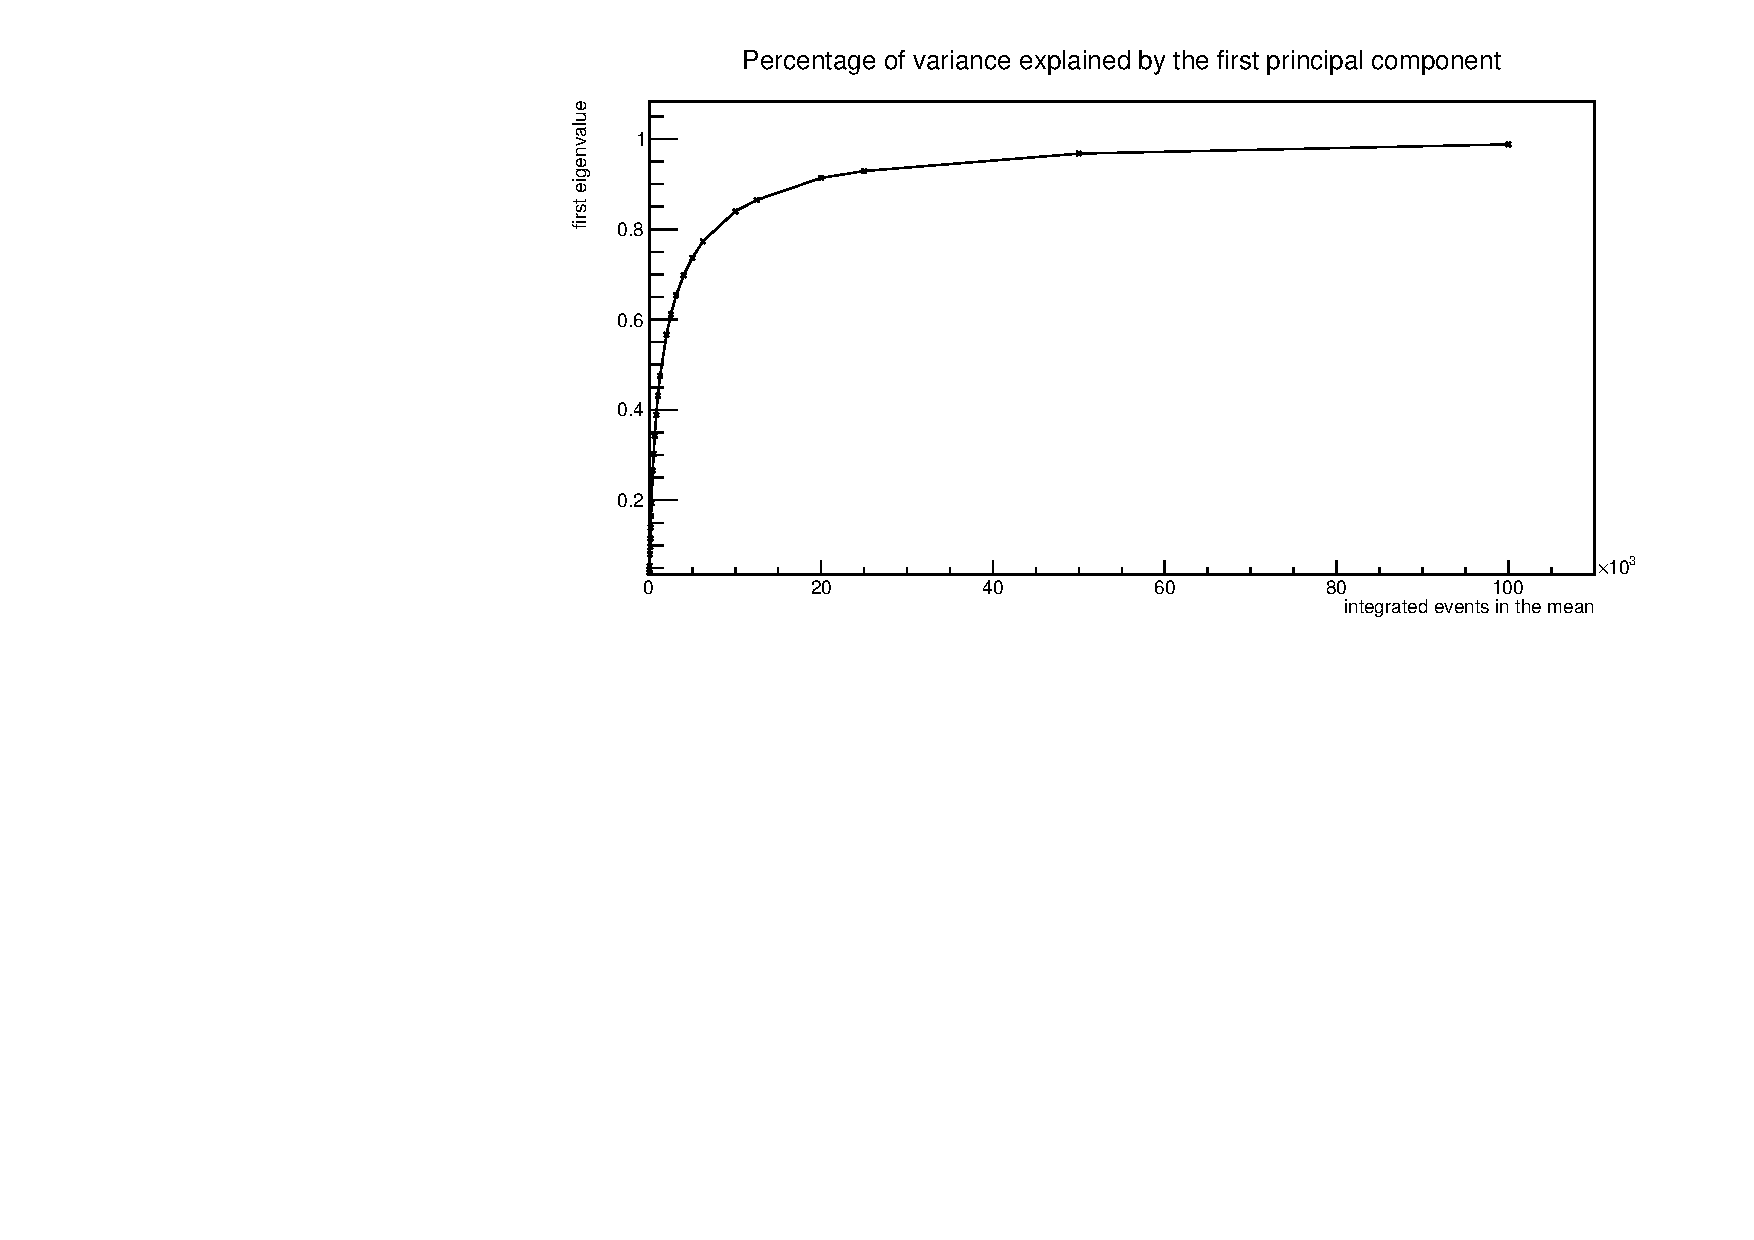
\includegraphics[width=\textwidth]{figures/explained_variance_new_y.pdf}
    \caption{Percentage of explained variance varying the number of integrated events for computing the mean number of clusters per event.}
    \label{fig:explained_variance}
\end{figure}


\begin{figure}
    \centering
    \begin{subfigure}{0.48\textwidth}
    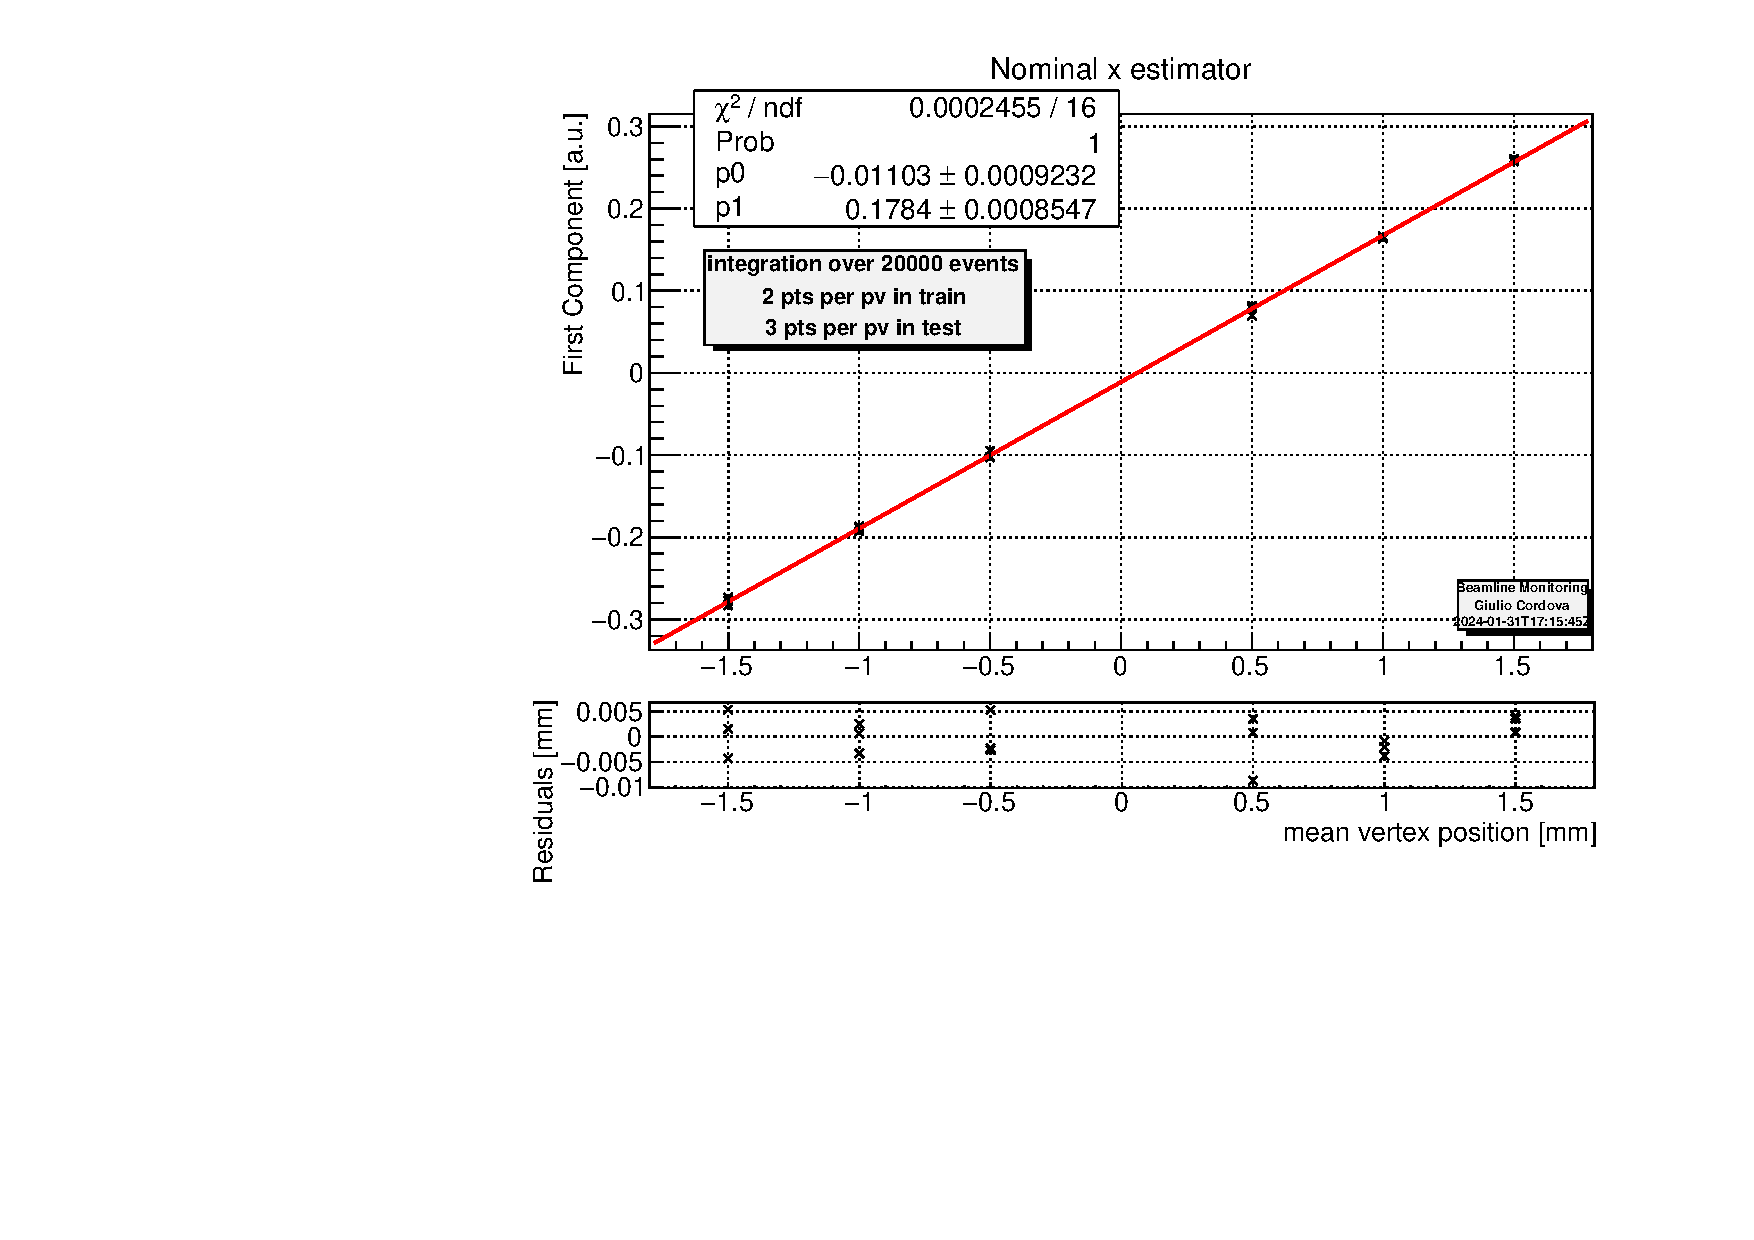
\includegraphics[width=\linewidth]{figures/x_fit.pdf}
    \caption{Linear Fit}\label{fig:xfit_MC}
    \end{subfigure}
    \begin{subfigure}{0.48\textwidth}
    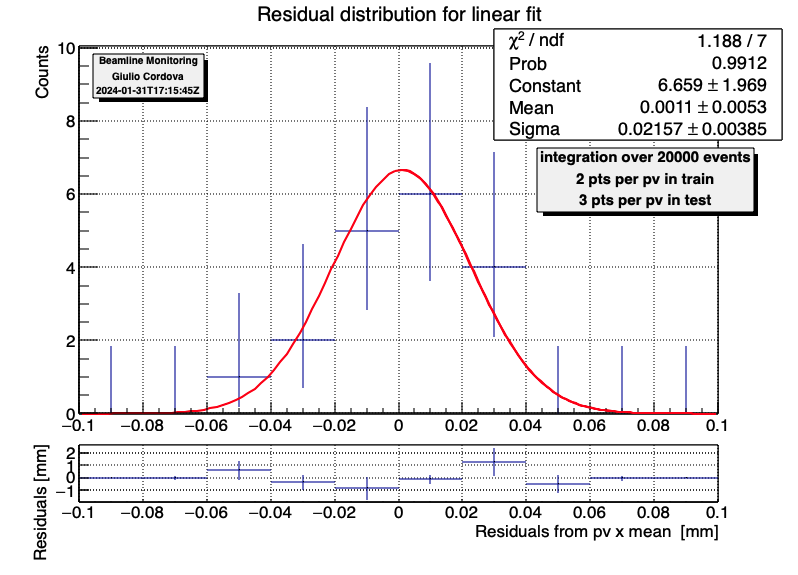
\includegraphics[width=\linewidth]{figures/x_res.png}
    \caption{Residuals from the fit}\label{fig:xres_Mc}
    \end{subfigure}
    \caption{Linearity of the first component calculated with the PCA with respect to beamline position shifts in x component}
    \label{fig:x_MC}
\end{figure}


\begin{figure}
    \centering
    \begin{subfigure}{0.48\textwidth}
    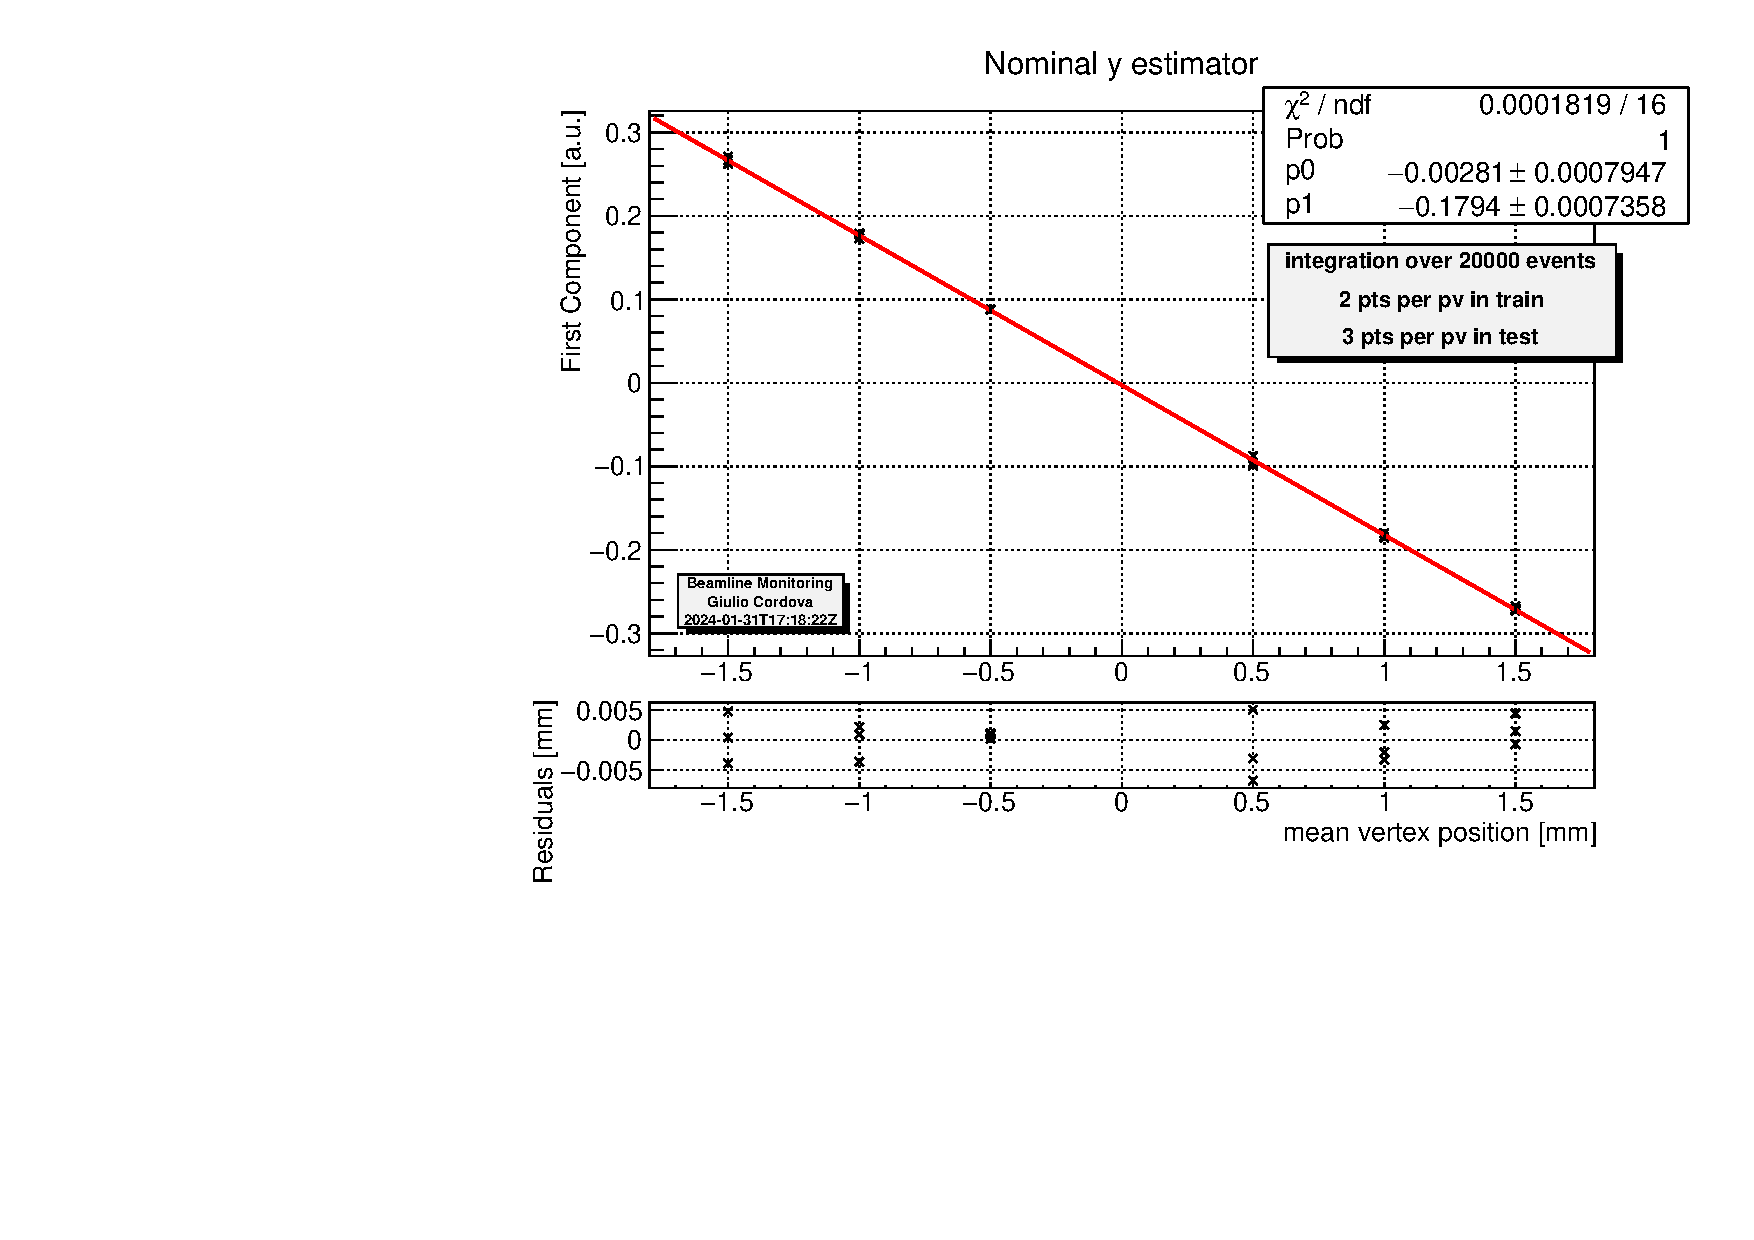
\includegraphics[width=\linewidth]{figures/y_fit.pdf}
    \caption{Linear Fit}\label{fig:yfit_MC}
    \end{subfigure}
    \begin{subfigure}{0.48\textwidth}
    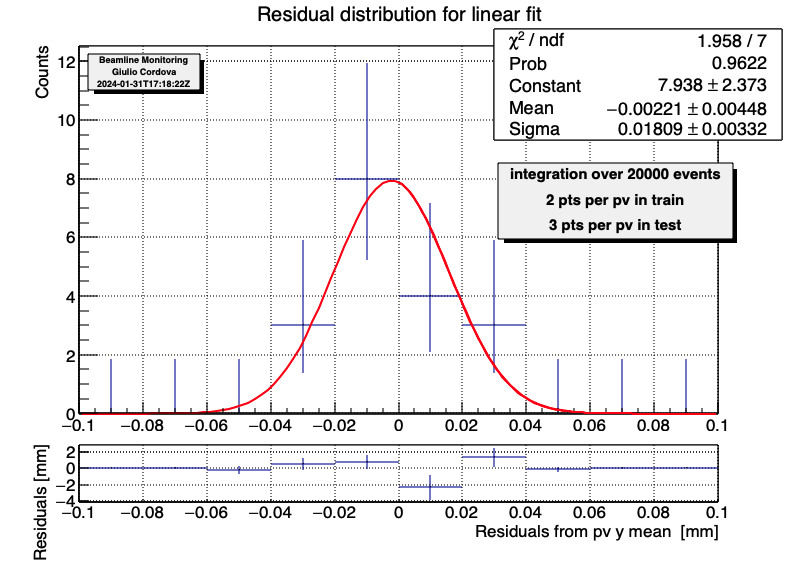
\includegraphics[width=\linewidth]{figures/y_res.png}
    \caption{Residuals from the fit}\label{fig:yres_MC}
    \end{subfigure}
    \caption{Linearity of the first component calculated with the PCA with respect to beamline position shifts in y component}
    \label{fig:y_MC}
\end{figure}


\begin{figure}
    \centering
    \begin{subfigure}{0.48\textwidth}
    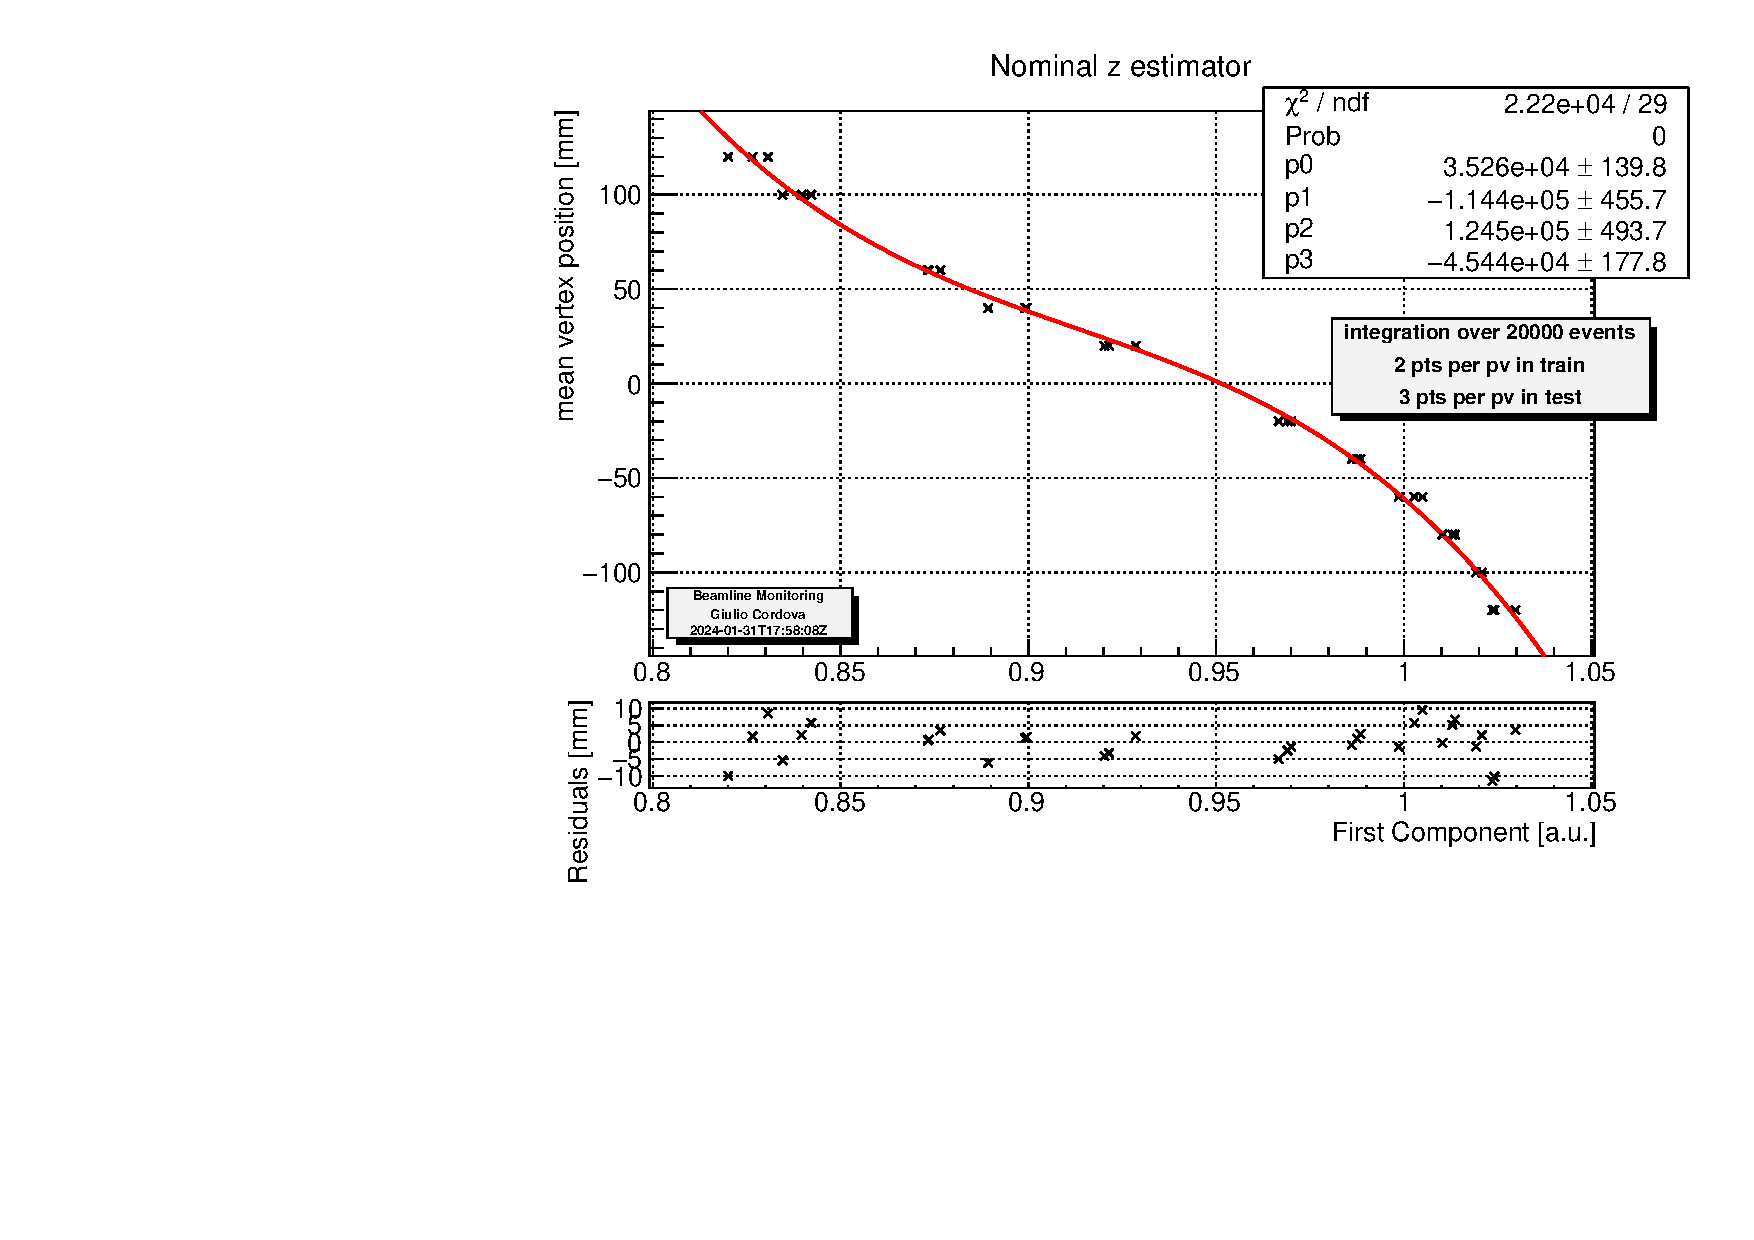
\includegraphics[width=\linewidth]{figures/z_cubic_fit.pdf}
    \caption{Cubic Fit}\label{fig:zfit_cubic_MC}
    \end{subfigure}
    \begin{subfigure}{0.48\textwidth}
    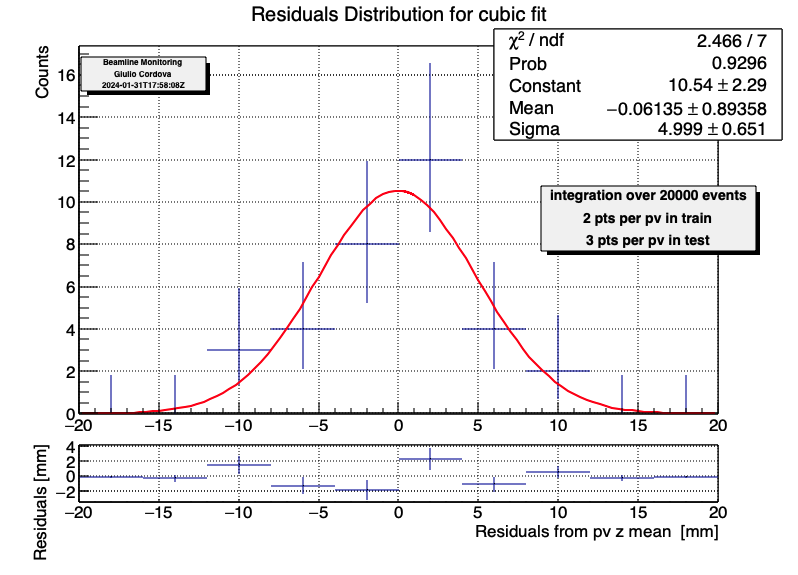
\includegraphics[width=\linewidth]{figures/z_cubic_res.png}
    \caption{Residuals from the fit}\label{fig:zres_cubic_MC}
    \end{subfigure}
    \caption{Cubic relationship between the first component calculated with the PCA and beamline position shifts in z component}
    \label{fig:z_cubic_MC}
\end{figure}



\begin{figure}
    \centering
    \begin{subfigure}{0.48\textwidth}
    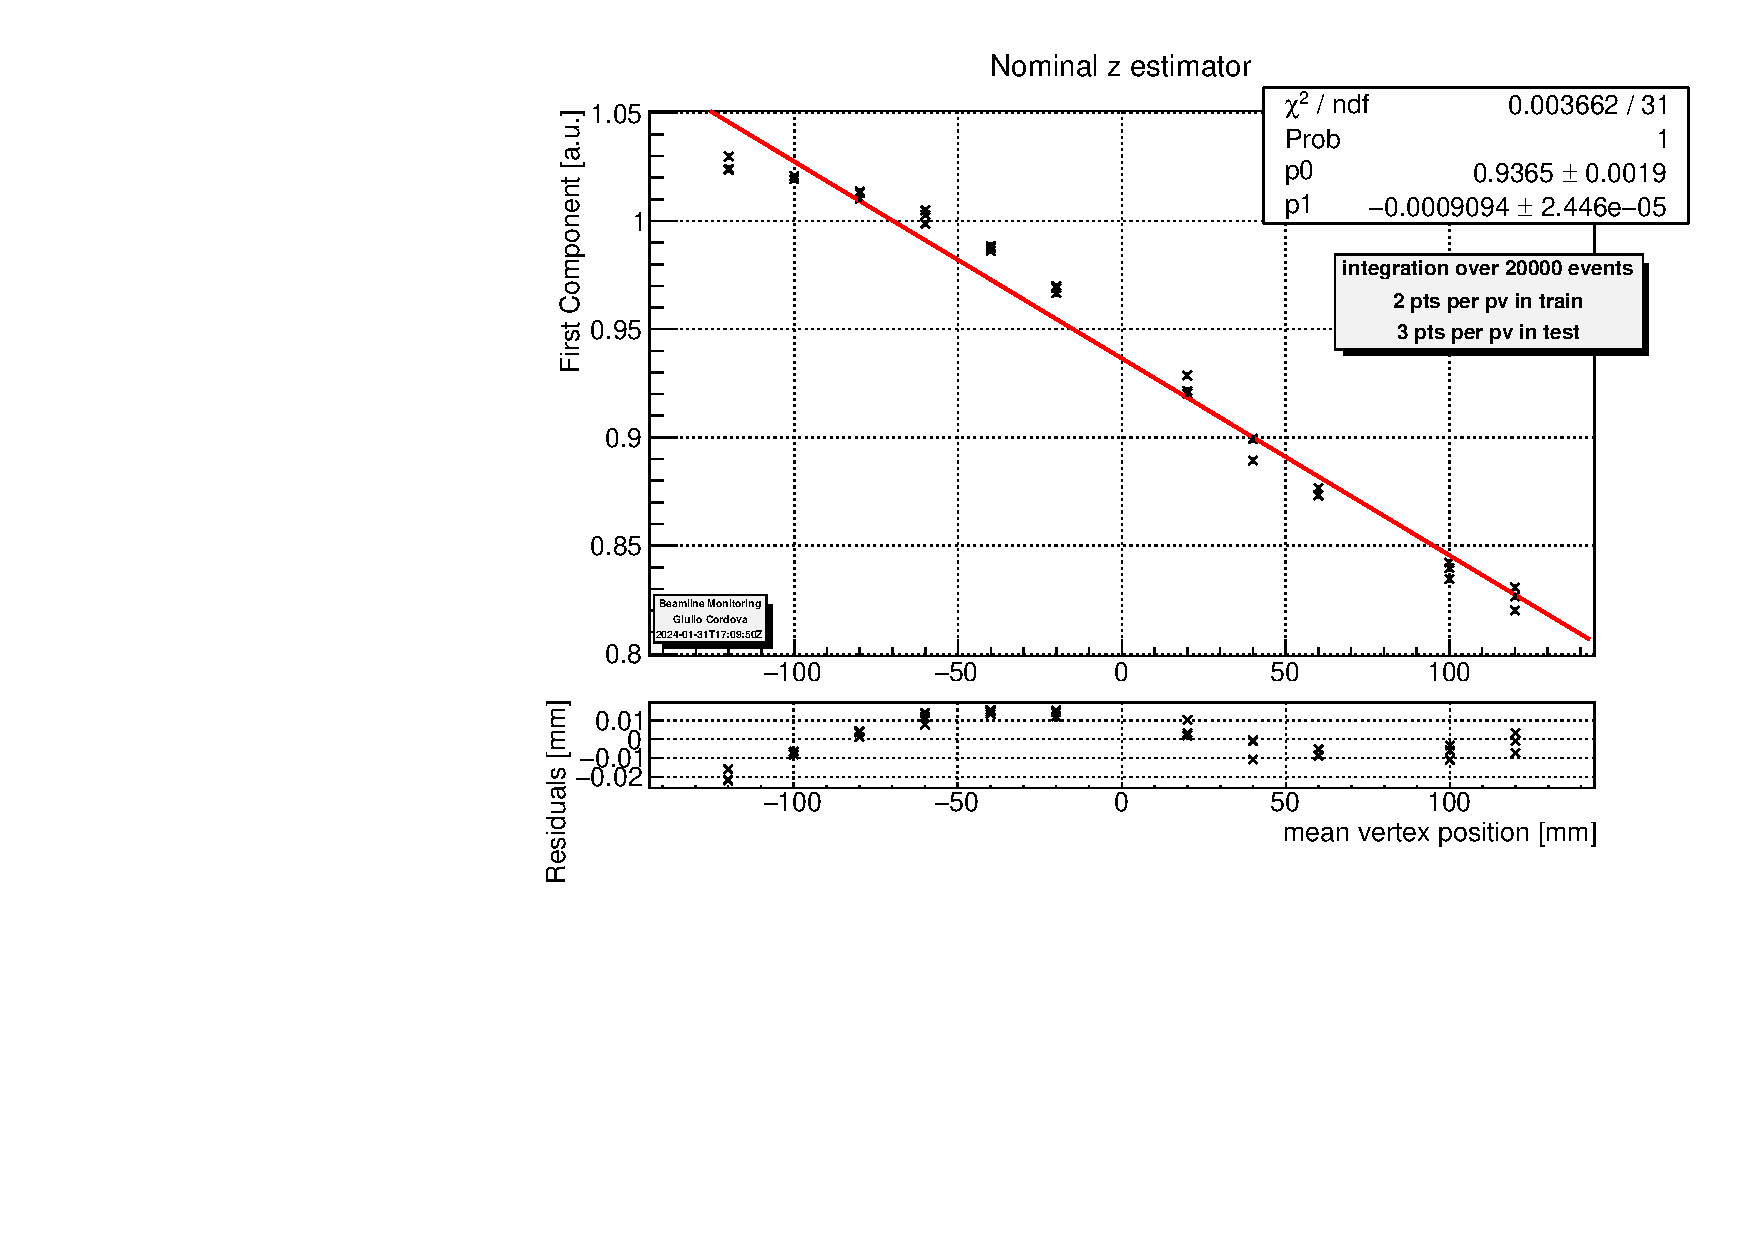
\includegraphics[width=\linewidth]{figures/z_fit.pdf}
    \caption{Linear Fit}\label{fig:zfit_MC}
    \end{subfigure}
    \begin{subfigure}{0.48\textwidth}
    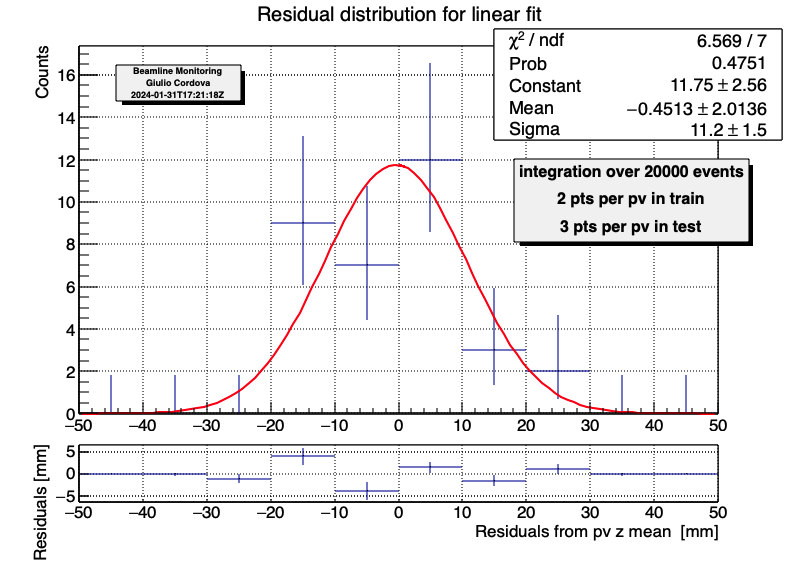
\includegraphics[width=\linewidth]{figures/z_res.png}
    \caption{Residuals from the fit}\label{fig:zres_MC}
    \end{subfigure}
    \caption{Linearity of the first component calculated with the PCA with respect to beamline position shifts in z component}
    \label{fig:z_MC}
\end{figure}


\section{Test on collision data}
\textit{Results obtained during VdM}

\section{Integration in LHCb online system}
\textit{qua ci metto i plot che si vedono nella pagina di Monet e spiego come li abbiamo implementati}
